\subsection{Анализ существующих аналогов}

На данный момент существует огромное множество программ для архивации данных. Какие-то из них имеют свои преимущества, какие-то -- свои недостатки.
В данном разделе рассматриваются наиболее известные и удобные приложения для сжатия и менеджмента файлов.

\subsubsection{WinRAR}

WinRAR -- это лицензионное программное обеспечение для сжатия данных различными способами. 
Программа хоть и лицензионная, но дает пробный период в 40 дней, по истечении которого пользователю снова предлагается приобрести лицензию.
Также на официальном сайте доступен защищенный авторскими правами исходный код распаковщика UnRAR, который позволяет его использовать не только в самом WinRAR, но и в других продуктах.

\begin{figure}[h]
    \centering
    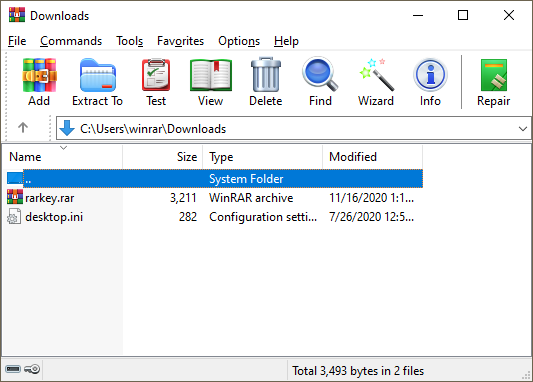
\includegraphics[width=0.85\linewidth]{\commonSecPathPrefix/sec_2/content/winrar.png}
    \caption{Программа WinRAR}
    \label{fig:WinRAR}
\end{figure}



Сам алгоритм сжатия основан на двух других алгоритмах: PPM и LZSS. 
Главная задумка PPM -- кодирование с помощью анализации данных и последующем предсказывании значения символов. 
Но основное сжатие в алгоритме PPM происходит с помощью усовершенствованного алгоритма Хаффмана. 
LZSS представляет собой словарный алгоритм основанный на алгоритме Лемпеля и Зива (LZ). 
Именно этот алгоритм послужил основой большинства современных приложений для архивации файлов.



Помимо архивов RAR программа поддерживает следующие файлы: ARJ, bz2, CAB, GZ, ISO, JAR, LZH, TAR, UUE, XZ, Z, ZIP, ZIPX, 7z.
Данный продукт обладает достаточно большим функционалом для работы с архивами и файлами, из-за чего в свою очередь он стал самым распространным приложением-архиватором в мире.


\subsubsection{7-Zip}

Программа 7-Zip является бесплатной и имеет открытый исходный код. 
Автором программы является Игорь Павлов -- российский разработчик, выпускник Уфимского государственного авиационного технического университета.
Основной формат архивации можно угадать из названия приложения -- 7z. 
Он имеет очень высокую степень сжатия благодаря использованию алгоритма LZMA (все тот же усовершенствованный Лемпеля и Зива -- LZ). 
Но при этом у пользователя нет возможности управлять файлом внутри архива и сжатые файлы данного формата не защищены от повреждений.

\begin{figure}[h]
    \centering
    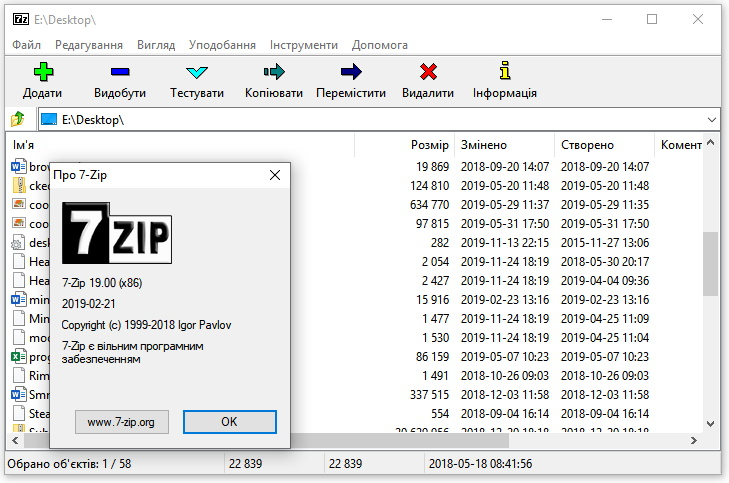
\includegraphics[width=0.85\linewidth]{\commonSecPathPrefix/sec_2/content/7zip.jpg}
    \caption{Программа 7-Zip}
    \label{fig:7zip}
\end{figure}



Кроме типа 7z архиватор имеет возможность упаковки и распаковки файлов: BZIP2 (BZ2, TB2, TBZ, TBZ2), GZIP (GZ, TGZ), TAR, ZIP, XZ, WIM.
А также только распаковка расширений типов:  ARJ, CAB, CHM, CPIO, CramFS, DEB, DMG, FAT, HFS, MBR, ISO, LZH, LZMA, MSI, NSIS, NTFS, RAR, RPM, SquashFS, UDF, VHD, XAR, Z.
Приложение 7-Zip из-за своей открытой лицензии позволяет устанавливать внешние плагины для работы с другими, непредусмотренными расширениями.



\subsubsection{WinZip}

Одним из первых архиваторов с графическим интерфейсом стал WinZip. 
Он был создан в начале 90-х и используется по сей день как основная программа-архиватор для Windows, macOS, IOS и Android.
WinZip как и WinRAR имеет платную лицензию.

\begin{figure}[h]
    \centering
    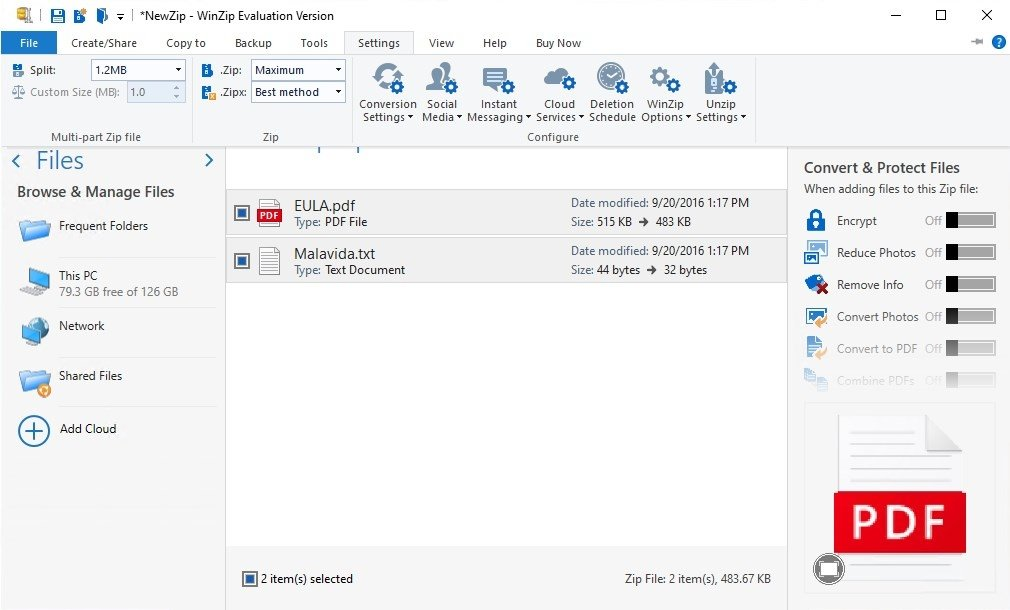
\includegraphics[width=0.85\linewidth]{\commonSecPathPrefix/sec_2/content/winzip.jpg}
    \caption{Программа WinZip}
    \label{fig:winzip}
\end{figure}



Данная программа может работать со следующими файлами: ZIP, tar, gzip, Z, Cabinet, RAR, bzip2, LHA, 7z, XZ, VHD и VMDK.
На данный момент WinZip поддерживает работу с облачными хранилищами, такими как Google Диск, SkyDrive, DropBox и другие.



Все вышеперечисленные программы обладают схожими функциями и очень широкими возможностями: от управления файлами в операционной системе до интеграций с облачными сервисами. 
Но даже такие разные программы по сути внутри имеют все ту же реализацию кода Хаффмана и алгоритма Лемпеля и Зива.
Поэтому, при сравнении конкурентов по скорости и степени сжатия данных, программы будут примерно равны по своим возможностям.
Главные отличия всех вышеперечисленных программ: дополнительные встроенные возможности приложений и их графический интерфейс. 
Здесь уже создатели приложений не ограничиваются фантазией и вставляют в приложения любой всевозможный функционал.



В этом курсовом проекте главная задача -- понять принцип действия предка современных способов сжатия данных -- алгоритма Хаффмана, осуществить на практике и спроектировать его в виде полноценного оконного приложения с графическим интерфейсом.